The whole framework could be mainly divided into four stages, lan pre-training , DiT pre-training, distance map training, and finally the inference stage.


In order to achieve accurate RNA-Distance predictions from vanilla Sequence


%\subsection{Se}

\subsection{RNA-FM Pre-Training}

The intention of this pre-training stage aims to provide rich RNA sequence representations for further downstream tasks as prescribed. A Bert-based language model with 12 transformer encoder blocks \cite{devlin2018bert} was trained on around 26 million non-coding RNA sequences in an unsupervised manner, where details could be found via another work [*]. After the training stage, a learned embedding layer will map an RNA sequence of Length $L$  to a $L\times 640$ tensor.

Noticed that this trained RNA Bert model could be applied directly for fine-tuning in other tasks. However, the difficulty of such an approach lies in the gap between enormous model capacity and relatively small downstream datasets. Thus, we reimplement a transformer-based downstream model DiT specified for tackling the distance prediction task.

\subsection{DiT pre-training}

F

\subsection{Distance Map Tuning}
DiT pre-training enbales 


\begin{figure*}[]
    \begin{center}
    %\caption{}\label{fig1}
    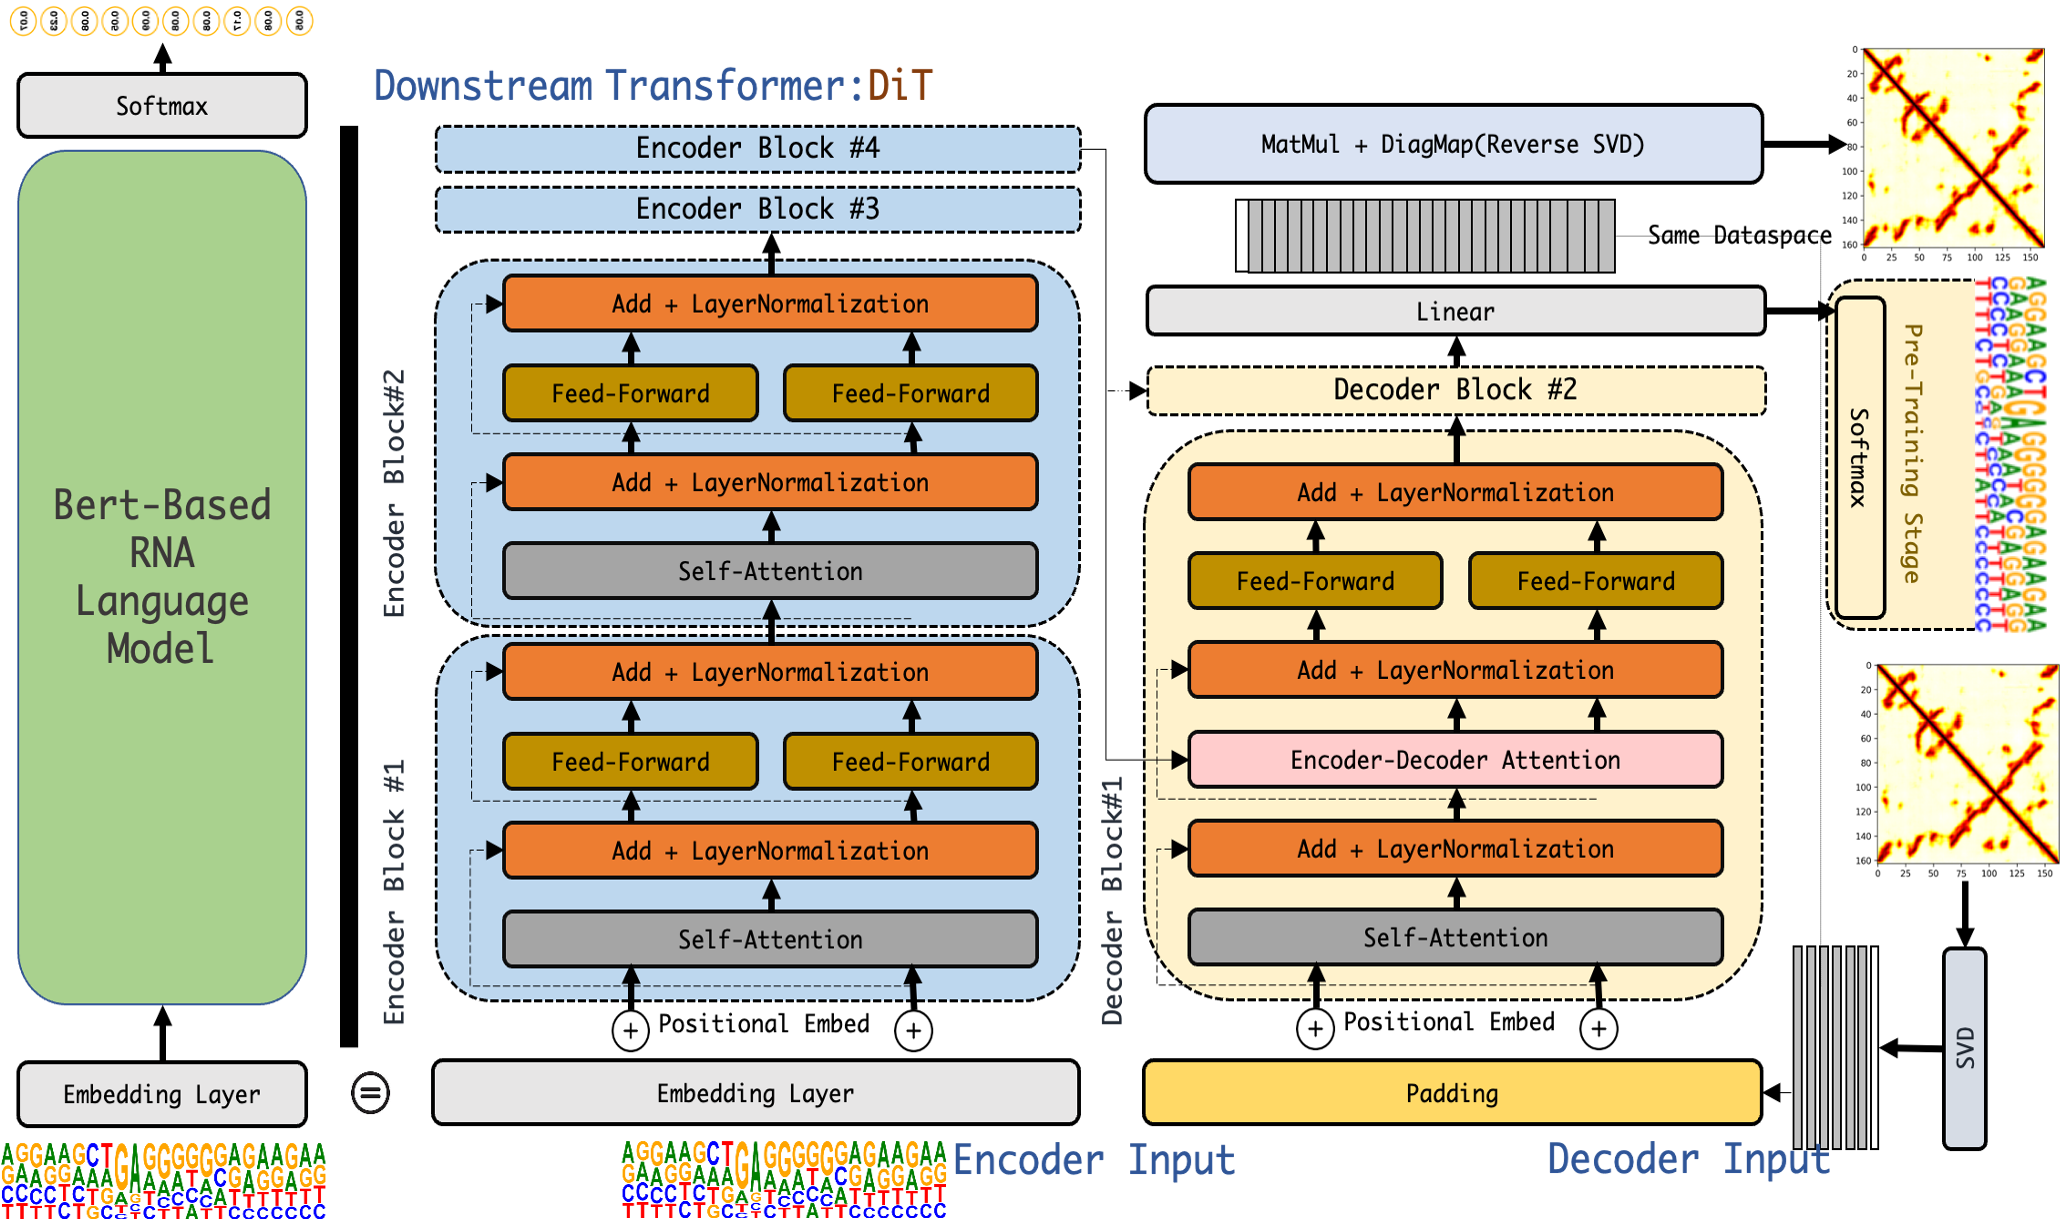
\includegraphics[width=1.0\textwidth]{1.png}
    \caption{Overview of the model's traininaag Stage}\label{Trainig Stage}
    \end{center}
\end{figure*}

\begin{figure*}[]
    \begin{center}
    %\caption{}\label{fig1}
    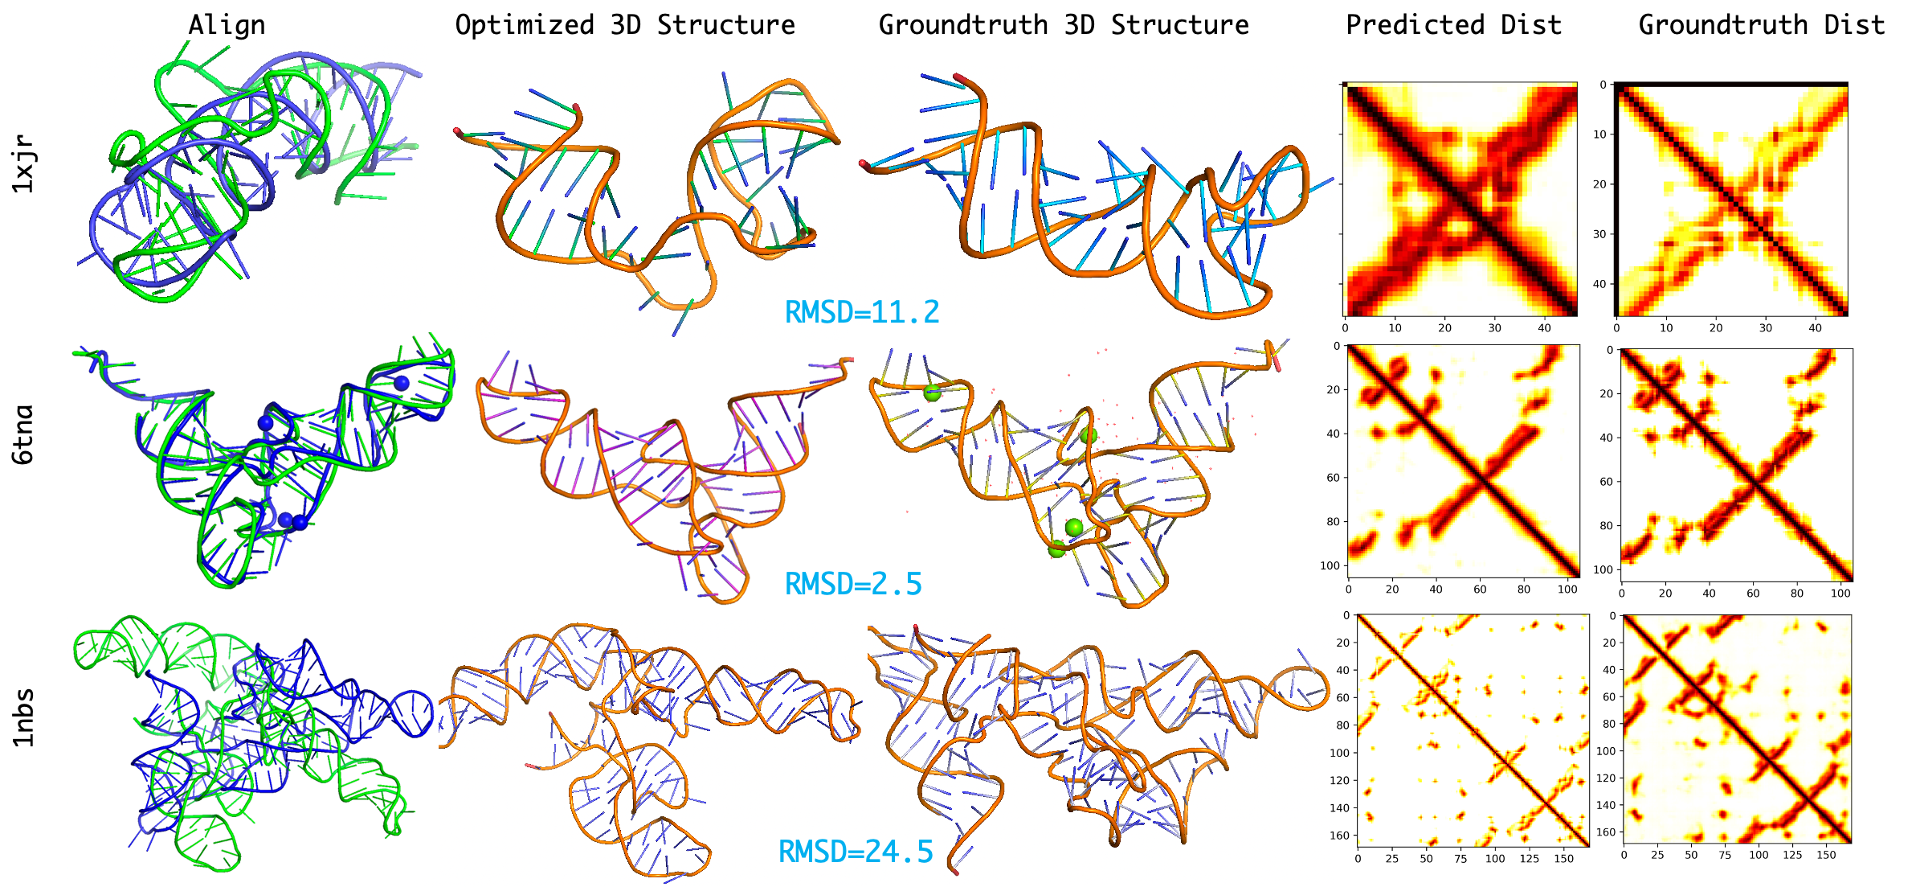
\includegraphics[width=1.0\textwidth]{2.png}
    \caption{Overview of the model'as training Stage}\label{Trainig Stage}
    \end{center}
\end{figure*}

\begin{figure*}[]
    \begin{center}
    %\caption{}\label{fig1}
    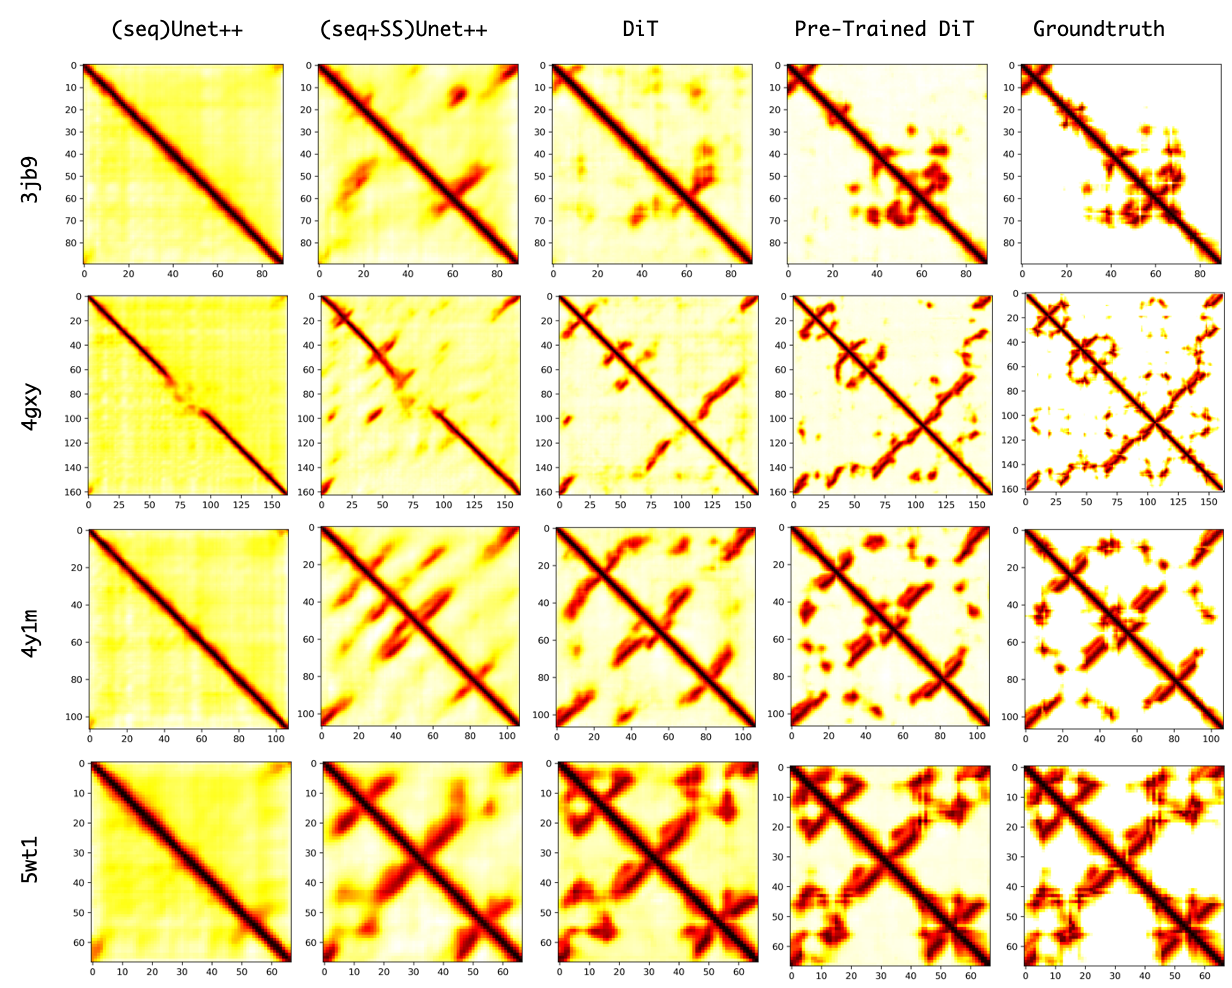
\includegraphics[width=0.8\textwidth]{3.png}
    \caption{Overview of the modelas's training Stage}\label{Trainig Stage}
    \end{center}
\end{figure*}
\begin{figure}[]
    \begin{center}
    %\caption{}\label{fig1}
    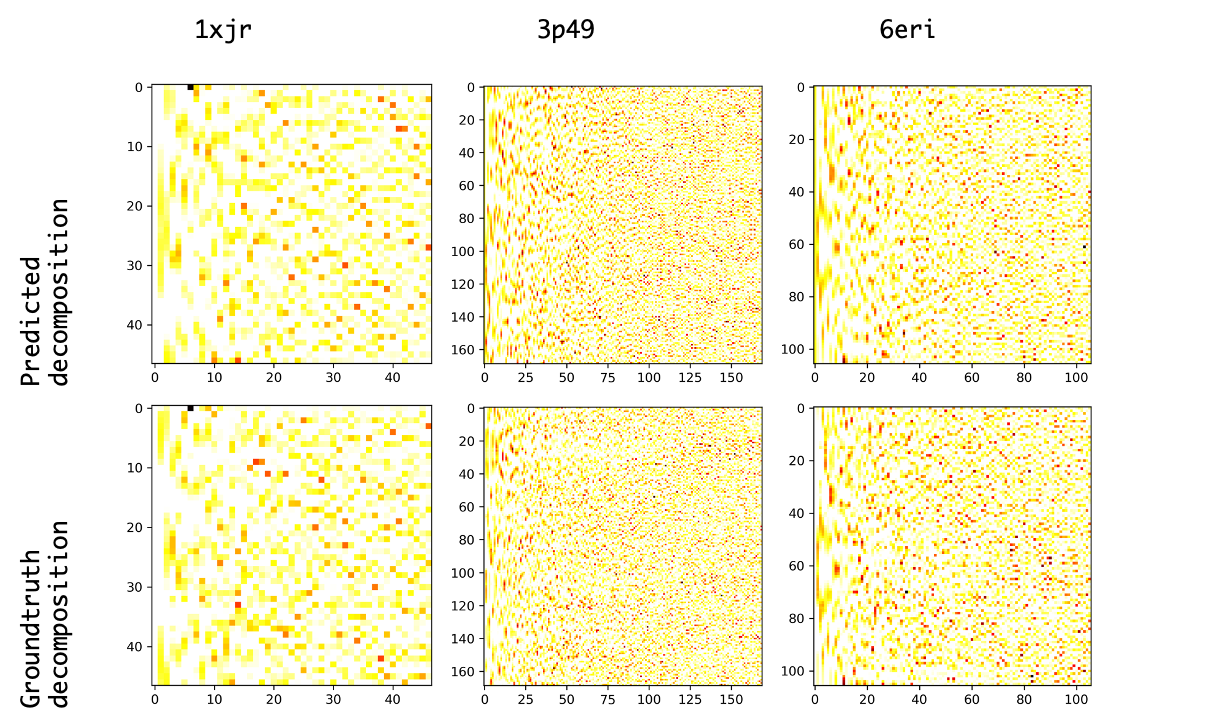
\includegraphics[width=0.5\textwidth]{svg.png}
    \caption{Overview of the modelas's training Stage}\label{Trainig Stage}
    \end{center}
\end{figure}
\begin{figure*}[]
    \begin{center}
    %\caption{}\label{fig1}
    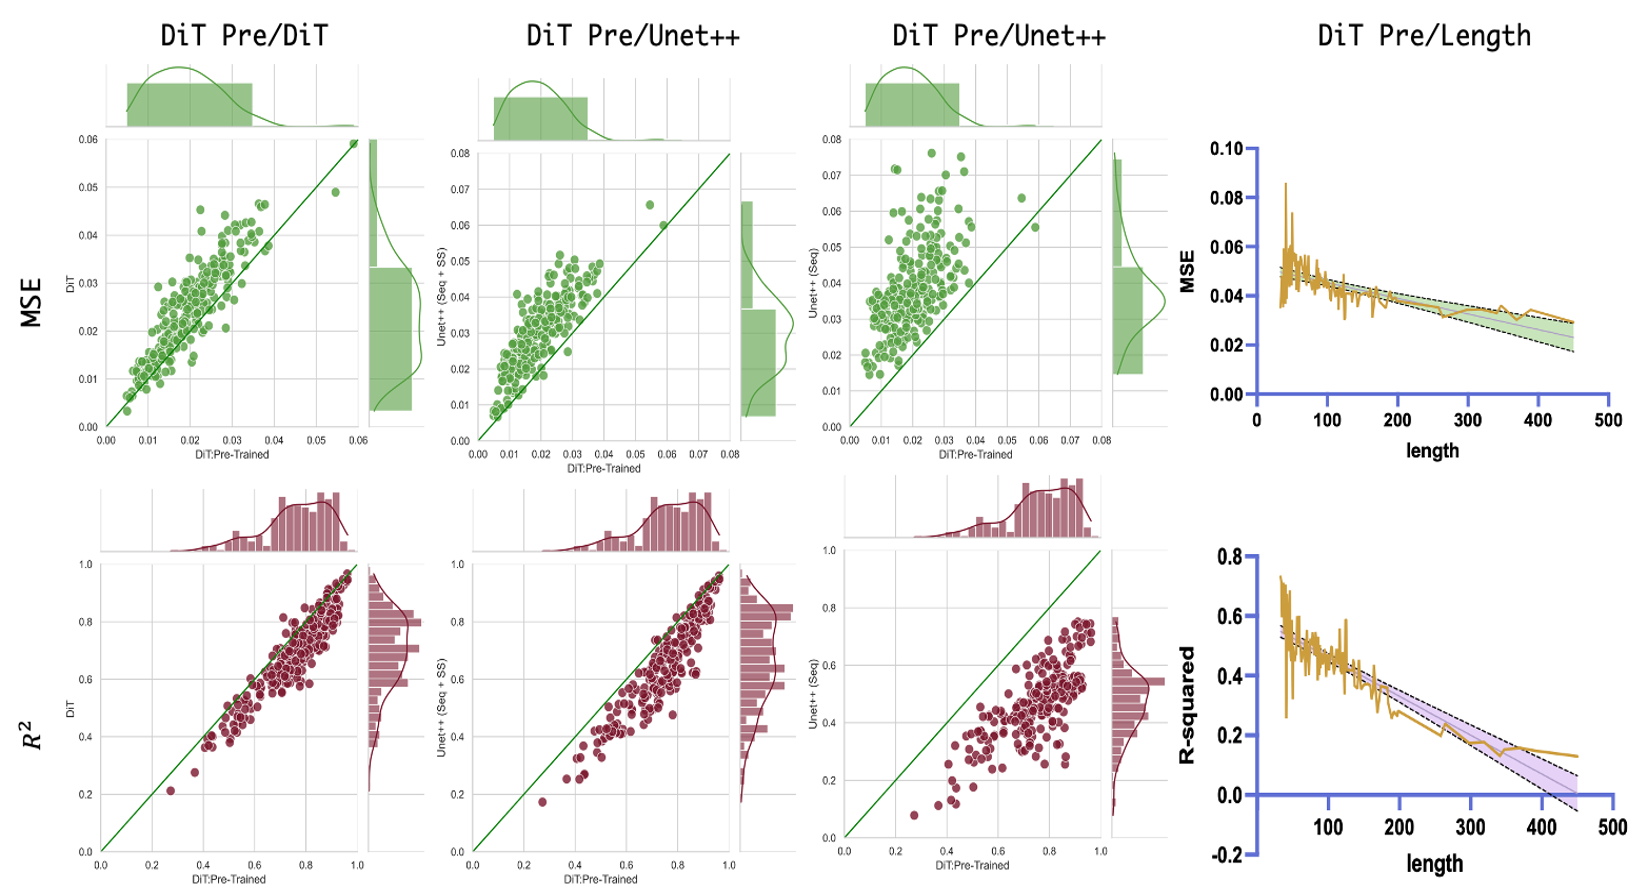
\includegraphics[width=1.0\textwidth]{4.png}
    \caption{Overview of the model's traiaaaaning Stage}\label{Trainig Stage}
    \end{center}
\end{figure*}


